\documentclass[12pt, a4paper]{article}
\usepackage{amssymb}
\usepackage{amsmath}
\usepackage{graphicx}
% \usepackage{authblk}
\usepackage{float}
\usepackage{subfig}
% \usepackage{epsfig}
% \usepackage{subfigure}
\usepackage{setspace}
\usepackage{geometry}
\geometry{left=2.5cm,right=2.5cm,top=2.5cm,bottom=2.5cm}

\usepackage{tabularx}
 
\title{COMP6706 Report: Towards More Accurate Fingerprint Recognition Using Deep Learning and Graph Matching}
\author{
    Cao Pei (20031287R) \\
    \text{peipei.cao@connect.polyu.hk}
    \and 
    Feng Yulin (18070059R) \\
    \text{yulin.feng@connect.polyu.hk}
}

% \renewcommand\Affilfont{\itshape\small}
% \author[1]{Cao Pei (20031287R)}
% \author[2]{Feng Yulin (18070059R)}
% \affil[1]{Hong Kong Polytechnic University}
% \affil[2]{Hong Kong Polytechnic University}
\date{}

\newcommand{\horrule}[1]{\rule{\linewidth}{#1}}
\newcommand{\entit}{COMP6706 Report: Towards More Accurate Fingerprint Recognition Using Deep Learning and Graph Matching}
\newcommand{\numword}{Number of Words: }

\begin{document}
\begin{titlepage}
    \begin{center}
        \horrule{0.5pt} \\ [0.4cm]
        \vspace{-1.5ex}
        { \bfseries \entit \\ \vspace{0.4cm}}
          \horrule{2pt} \vspace{-2ex}
        \numword \\
    \end{center}

    \vspace{3cm}
    \begin{table}[h]
        \centering
        \begin{tabular}{p{3cm}<{\raggedleft} p{6cm}<{\centering}}
          Name: & {Cao Pei}            \\
          Student ID: & {20031287R}          \\
          Email: & {peipei.cao@connect.polyu.hk} \\
        \end{tabular}
    \end{table}

    \vspace{3cm}
    \begin{table}[h]
        \centering
        \begin{tabular}{p{3cm}<{\raggedleft} p{6cm}<{\centering}}
          Name: & {Feng Yulin}            \\
          Student ID: & {18070059R}          \\
          Email: & {yulin.feng@connect.polyu.hk} \\
        \end{tabular}
    \end{table}

\end{titlepage}

\newpage

\begin{spacing}{1} 
    % \maketitle   

    \begin{abstract}
    hahahah
    \end{abstract}

    \section{Introduction}
    Fingerprint used for human identification can be dated back to over one hundred years ago when people found that no two individuals shared the same fingerprints. Fingerprint was used in forensics  since criminals usually unintentionally left their fingerprints in crime scenes and their fingerprints can be used as evidence against themselves. These applications calls for the use of fingerprint and thus research on fingerprint recognition. Compared with other biometrics such as face, iris and voice, fingerprint is highly distinctive, permanent, easy to accept and easy to collect \cite{Maltoni2009}. This makes fingerprint one of the most popular biometrics which is used in a large number of recognition domains such as healthcare, electronic payment and border crossing.
    
    Because manual fingerprint recognition requires human experts to match fingerprint one by one, the cost of training such experts is high, and matching fingerprint with fingerprints in the database is time consuming and slow, the demand for automatic fingerprint recognition is growing quickly. This makes fingerprint recognition a popular pattern recognition research problem. Although many fingerprint recognition solutions have been proposed and showed their effectiveness over the past few decades, fingerprint recognition is still challenging especially for low quality fingerprints due to fingerprint noise and distortion. Therefore, it is an intriguing  research problem even till nowadays, and accurate and fast fingerprint recognition algorithm is in demand.
    
    Fingerprint recognition, also called fingerprint matching, can basically be divided into two categories: minutiae based matching and non-minutiae based matching. Minutiae is considered as stable and robust local fingerprint ridge characteristics. Minutiae is usually represented by location, orientation, and minutiae type (i.e., ridge endings and ridge bifurcations). Therefore, minutiae based matching methods try to align two fingerprints by matching the largest number of corresponding minutiae pairs. For low quality fingerprint when it is difficult to extract minutiae, non-minutiae based matching comes into play. Some other fingerprint features such as ridge orientation, ridge frequency,  and ridge shape. To date, most fingerprint recognition algorithms are based on minutiae because of its stability and robustness.
    
    Conventional minutiae based fingerprint recognition method considers matching minutiae pairs by comparing minutiae between two fingerprints. The fast development and increasing popularity of deep learning methods shows remarkable progress in computer vision tasks. Some challenging biometric problems, such as face recognition \cite{SchroffCVPR2015facenet} and iris recognition \cite{ZhaoICCV2017}, have achieved great success thanks to deep learning based methods. There are also some works on using deep learning based methods for fingerprint matching and research shows that deep learning method can also improve fingerprint matching in some scenarios. As another popular research area, graph neural network has also made significant progress over the last decade. Since minutiae of one fingerprint can be formulated as a graph, this implies the possibility of applying graph neural network for matching minutiae graphs. 
    
    Conclusions are in Section \ref{sec:conclusion}.


    \section{Related Work}
    \label{sec:related}

    \subsection{Conventional Fingerprint Recognition Method}
    Minutiae based method is the most widely used method for fingerprint recognition. Consider two fingerprint images with M and N minutiae respectively. Each minutiae is represented by location, orientation and type. A solution is required to match as many minutiae pairs as possible. To achieve this goal, local minutiae structures are formed to match minutiae. Compared with global minutiae matching \cite{ChikkerurICB2006}, local minutiae matching are computationally cheaper and more robust against fingerprint distortion. Earlier approaches can be found in \cite{HrechakPR1990} and \cite{KovacsTPAMI2000}. To describe local minutiae structure, two methods were proposed: nearest neighbor based and fixed radius based. For nearest neighbor based method, the number of neighbors is fixed \cite{JiangICPR2000} so each minutiae has same number of nearest neighbors. For fixed radius method, a radius is given so that all minutiae that fall within the circle defined by the minutiae as the center and the radius are included \cite{CappelliTPAMI2010mcc}. However, both approaches have their own drawbacks. Nearest neighbor method suffers from missing minutiae and spurious minutiae. Although fixed length method alleviates the issue of missing minutiae and spurious minutiae, it has potential border issues, which means that the minutiae near the border of the circle should be properly treated.

    \subsection{Deep Learning Method for Fingerprint Recognition}
    The past decade has witnessed the great progress of deep learning in computer vision and pattern recognition \cite{HeCVPR2016ResNet} \cite{Simonyan2014VGG} \cite{SzegedyCVPR2015InceptionV1}. The name “deep learning” is derived from the architecture of deep artificial neural networks, which belongs to the family of machine learning methods. Compared with traditional neural networks which have only one or two layers, deep neural network can have tens or hundreds of layers. Such great progress of deep learning has also facilitated not only the research on fingerprint matching \cite{CaoTPAMI2018}, but also the research on other fingerprint recognition related tasks, such as minutia extraction \cite{TangIJCB2017} \cite{NguyenICB2018}. \cite{LinTIFS2018} did the pioneering work on matching with contactless and contact-based 2D fingerprint with convolutional neural network (CNN), while \cite{LinPR2018} also used CNN to match 3D fingerprint, and both works showed that fingerprint recognition with CNN based method can achieve outperforming results. Instead of extracting minutiae for fingerprint matching, \cite{EngelsmaTPAMI2019} trained a deep neural network to extract fixed-length fingerprint descriptor and regarded minutiae extraction as one step to achieve the final fixed-length representation.

    \subsection{Graph Neural Network}
    Minutiae of one fingerprint can be formulated as a graph by connecting each minutiae based on some predefined rules. However, due to fingerprint noise and distortion, minutiae graph matching can achieve as good performance as other minutiae based matching method \cite{ChikkerurICB2006}. There is another related research area called graph neural network (GNN).The success of deep neural networks has also boosted the research on graph neural network  in recent years \cite{WuTNNLS2020} \cite{ZhouAI2020} \cite{XuICLR2019GIN}. Compared with images that are structured data, there are also unstructured data in the real world, such as social networks, molecules, and citation networks. Deep neural networks have some limitations to model such kind of data, but graph neural networks show their own flexibility. Motivated by CNN, there is a similar graph convolutional networks called GCN \cite{KipfICLR2017}. A graph is represented by nodes and edges. For classification task, it can be divided in to node level based classification and graph level based classification. GNN can also be used for graph matching \cite{ZanfirCVPR2018} \cite{LiICML2019}. Graph matching is an NP-hard problem, and thus requires complex matching algorithm. \cite{SarlinCVPR2020superglue} formulated graph matching as optimal transport problem which can be solved an efficient approximation algorithm called Sinkhorn algorithm \cite{CuturiNIPS2013sinkhorn}. 
    
    \section{Methods}
    \label{sec:method}


    \section{Experimental Results}
    \label{sec:experiment}


    \section{Minutiae Graph}
    Vertex is represented by the minutiae location $(x, y)$. For the edge configuration, there are two ways to connect the vertices by edges. One way is to connect each vertex with its $k$ nearest neighbor where the number $k$ is preset by the user. However, this method is sensitive to missing or spurious minutiae. The other way is connect the vertices by Delaunay triangulation.

    % \begin{figure}[htb]
    %     \begin{minipage}[b]{0.48\linewidth}
    %         \centering
    %         \centerline{\epsfig{figure=mnt_overlay.png, width=4.0cm}}
    %         \caption{Minutiae}
    %         \label{fig:mnt_over}
    %     \end{minipage}
    %     \hfill
    %     \begin{minipage}[b]{0.48\linewidth}
    %         \centering
    %         \centerline{\epsfig{figure=triangulation.png, width=4.0cm}}
    %         \caption{Triangulation}
    %         \label{fig:triang}
    %     \end{minipage}
    % \end{figure}


    % \begin{figure}[htb]
    % \centering
    % \subfigure[Minutiae]{\epsfig{figure=./image/fingerprint1_1/mnt_overlay.png, height=4.0cm}}
    % \hspace{0in}
    % \subfigure[Triangulation]{\epsfig{figure=./image/fingerprint1_1/triangulation.png, width=4.0cm, height=4.0cm}}
    % \hspace{0in}
    % \subfigure[Triangulation]{\epsfig{figure=./image/fingerprint1_1/mnt_graph.png, width=4.0cm, height=4.0cm}}
    % \caption{Fingerprint1_1}
    % \label{fig:fingerprint1_1}
    % \end{figure}

    
    \begin{figure*}[!ht]
        \centering
        \begin{minipage}[b]{0.93\linewidth}
            \subfloat[minutiae]{
                \begin{minipage}[b]{0.27\linewidth}
                    \centering
                    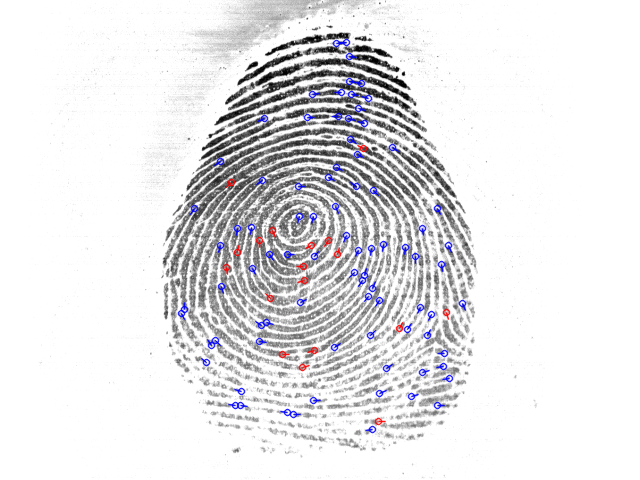
\includegraphics[height=4.0cm]{./image/fingerprint1_1/mnt_overlay.png}\vspace{8pt}
                    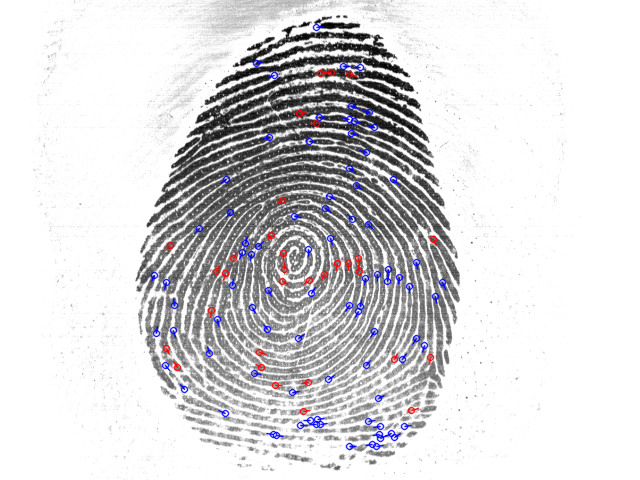
\includegraphics[height=4.0cm]{./image/fingerprint1_2/mnt_overlay.png}\vspace{8pt}
                    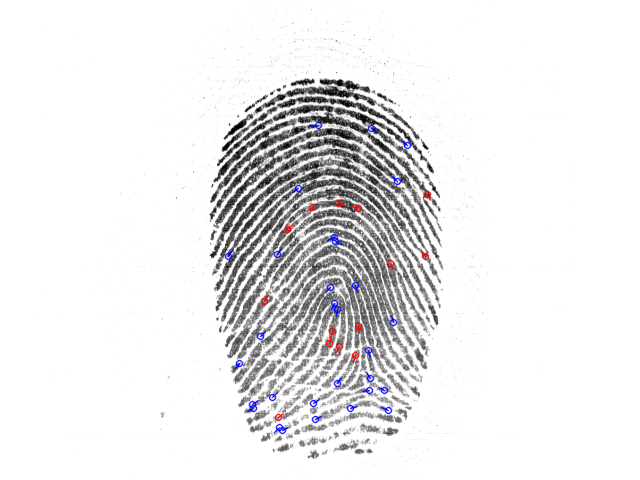
\includegraphics[height=4.0cm]{./image/fingerprint2_1/mnt_overlay.png}
                \end{minipage}
            }
            \hfill
            \subfloat[triangulation]{
                \begin{minipage}[b]{0.27\linewidth}
                    \centering
                    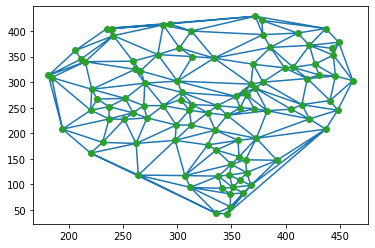
\includegraphics[width=\linewidth, height=4.0cm]{./image/fingerprint1_1/triangulation.png}\vspace{8pt}
                    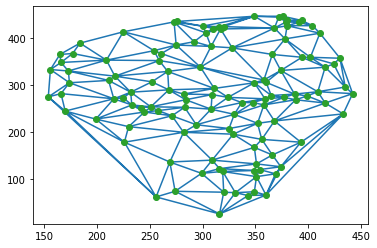
\includegraphics[width=\linewidth, height=4.0cm]{./image/fingerprint1_2/triangulation.png}\vspace{8pt}
                    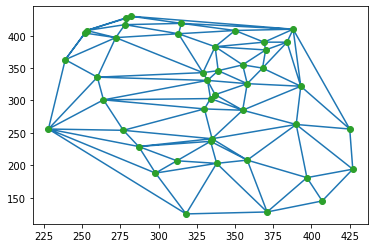
\includegraphics[width=\linewidth, height=4.0cm]{./image/fingerprint2_1/triangulation.png}
                \end{minipage}
            }
            \hfill
            \subfloat[graph]{
                \begin{minipage}[b]{0.27\linewidth}
                    \centering
                    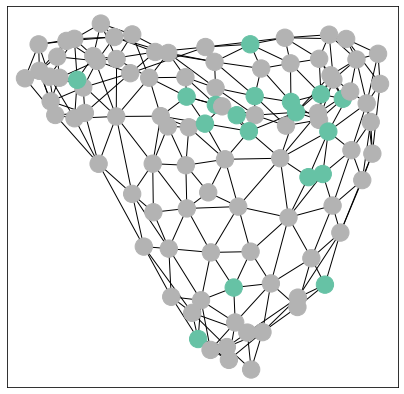
\includegraphics[width=\linewidth, height=4.0cm]{./image/fingerprint1_1/mnt_graph.png}\vspace{8pt}
                    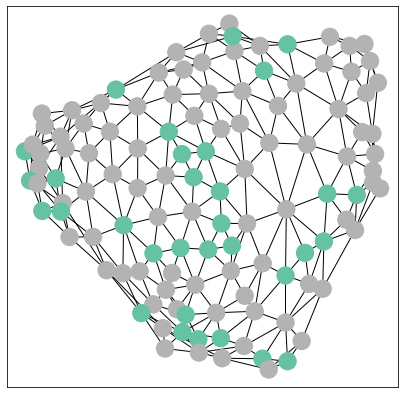
\includegraphics[width=\linewidth, height=4.0cm]{./image/fingerprint1_2/mnt_graph.png}\vspace{8pt}
                    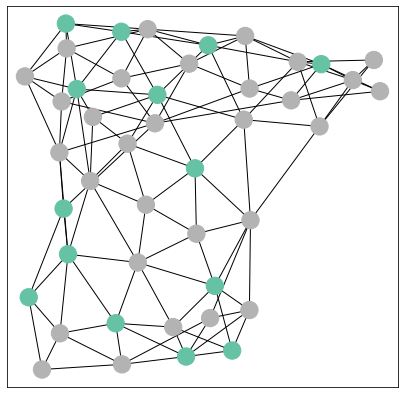
\includegraphics[width=\linewidth, height=4.0cm]{./image/fingerprint2_1/mnt_graph.png}
                \end{minipage}
            }
        \end{minipage}
        \vfill
        \caption{Fingerprint}
        \label{fig:mnt}
    \end{figure*}

    The left column shows the original fingerprint with detected minutiae that are plotted on it. The middle column shows the minutiae that are connected by Delaunay triangulation method. Note that because the origin of the fingerprint image is on the top left and the origin of the plot is on the bottom left, the minutiae that are plotted in the middle column are turned upside down compared with those minutiae in the left column. The right column shows the minutiae graph once the vertices and edges are built from the previous two columns. The geometric information of the minutiae is lost in the minutiae graph. 

    \section{Graph Triplet}
    We use MNIST dataset \cite{LecunIEEE1998} to build the graph triplet, and use SplineCNN layer \cite{FeyCVPR2018splinecnn} \cite{FeyICLR2020DGMC} to replace the CNN layer which is normally used in computer vision task. Each MNIST image is represented as a graph, whose nodes correponds to the pixels in the image and the edge is formed by connected each pixel to all its neighboring pixels. Therefore, based on this setup, each MNIST image is a graph with the same number of nodes, which is $784(=28^2)$. The graph triplet is formulated as followes: for each sample as the anchor in the training dataset, we randomly select another sample which belongs to the same class as the positive sample, and randomly select one sample from the rest classes as the negative sample. 
    
    Similar to CNN neural network configuration, we build a SplineCNN network, which contains two SplineCNN layers, and ech SplineCNN layer is followed by an exponentail linear unit (ELU) and a maxpooling layer. There are two fully connected layers, the first fully connected layer is also followed by an ELU layer, the output dimension of the final fully connected layer is $10$ (we also choose the final dimension to be $2$ for visualization). The initial learning rate is $10^{-3}$. Stochastic gradient descent with Adam method is used for optimization and the total training epochs is $20$.

    For evaluation, since the total number of samples of MNIST test dataset is $10,000$ and they are not balanced for each class, we randomly choose 500 samples from each class. We use all-to-all evaluation protocal, which means for each test sample, Euclidean distance is computed against all the rest samples. Therefore, in total, we generate $1,247,500$ genuine scores and $11,250,000$ impostor scores. Since MNIST dataset is a simple dataset with a few number of classes and a large number of samples for each class, it turns out that there is no overlap between genuine scores and impostor scores. The equal error rate(EER) is thus zero.

    \section{Conclusion and Future Work}
    \label{sec:conclusion}

       


\bibliographystyle{plain}
\bibliography{ref}

\end{spacing}
\end{document}

 